\section{Introduction}
\label{sec:intro}

Over the last decade, microcontrollers, the workhorses of embedded systems, have become 
central to efforts in making and education. For example, the Arduino project 
(\url{www.arduino.cc})~\cite{buildingArduino2014}, 
started in 2003, created the Uno using an 8-bit Atmel 
AVR microcontroller. The Uno makes most of its microcontrollers I/O pins available via headers;
external hardware modules (shields) may be connected to these headers to extend 
its capability.    The Arduino ecosystem has grown tremendously in the past 15 years, 
with the support of companies such as Adafruit Industries (\url{www.adafruit.com}) and 
Sparkfun Electronics (\url{www.sparkfun.com}).

What has not changed much is the way microcontrollers are programmed,
which is with the C and C++ programming languages, as well as assembly.   
This is not a huge surprise, given the low-level nature of microcontroller programming, 
where direct access to the hardware is needed. There generally is no operating 
system running on such boards, as they have very little RAM (2K for the Uno, for example) and 
lack memory protection hardware. What is more surprising about the Arduino platform is that:
\begin{itemize}
\item it encourages the programmer to use polling to interact with sensors, 
leading to monolithic sequential programs;
\item its IDE lacks any code ``intellisense'' or common interactive features of modern IDEs;
\item it loads code onto the microcontroller using 1980s era bootloader technology.
\end{itemize}
As a result, it is not simple to get started with Arduino systems, of which there are many. 
On the other hand, on the web we find many excellent environments for introductory programming. 
Visual block editors such as Scratch (\url{https://scratch.mit.edu/})~\cite{ScratchCACM2009,BlocksBeyondCACM2017} 
and Blockly (\url{https://developers.google.com/blockly/})~\cite{Blocky2015}
allow the creation of programs without the possibility of syntax errors. 
HTML, CSS and JavaScript allow a complete programming experience to be delivered as an interactive 
web app, including editing with intellisense, code execution and debugging~cite{Monaco}.
The programming models associated with Scratch and Blockly generally are 
event based, freeing the programmer from the need to poll.

We have created a new programming platform that bridges the worlds of the microcontroller
and the web app. The major goals of the platform are to: (1)
make it simple to program microcontrollers using nothing more than a web app;
(2) allow a user's compiled program to be easily installed on a microcontroller;
(3) enable the safe addition of new of software/hardware components to a microcontroller.

\begin{figure*}[t]
  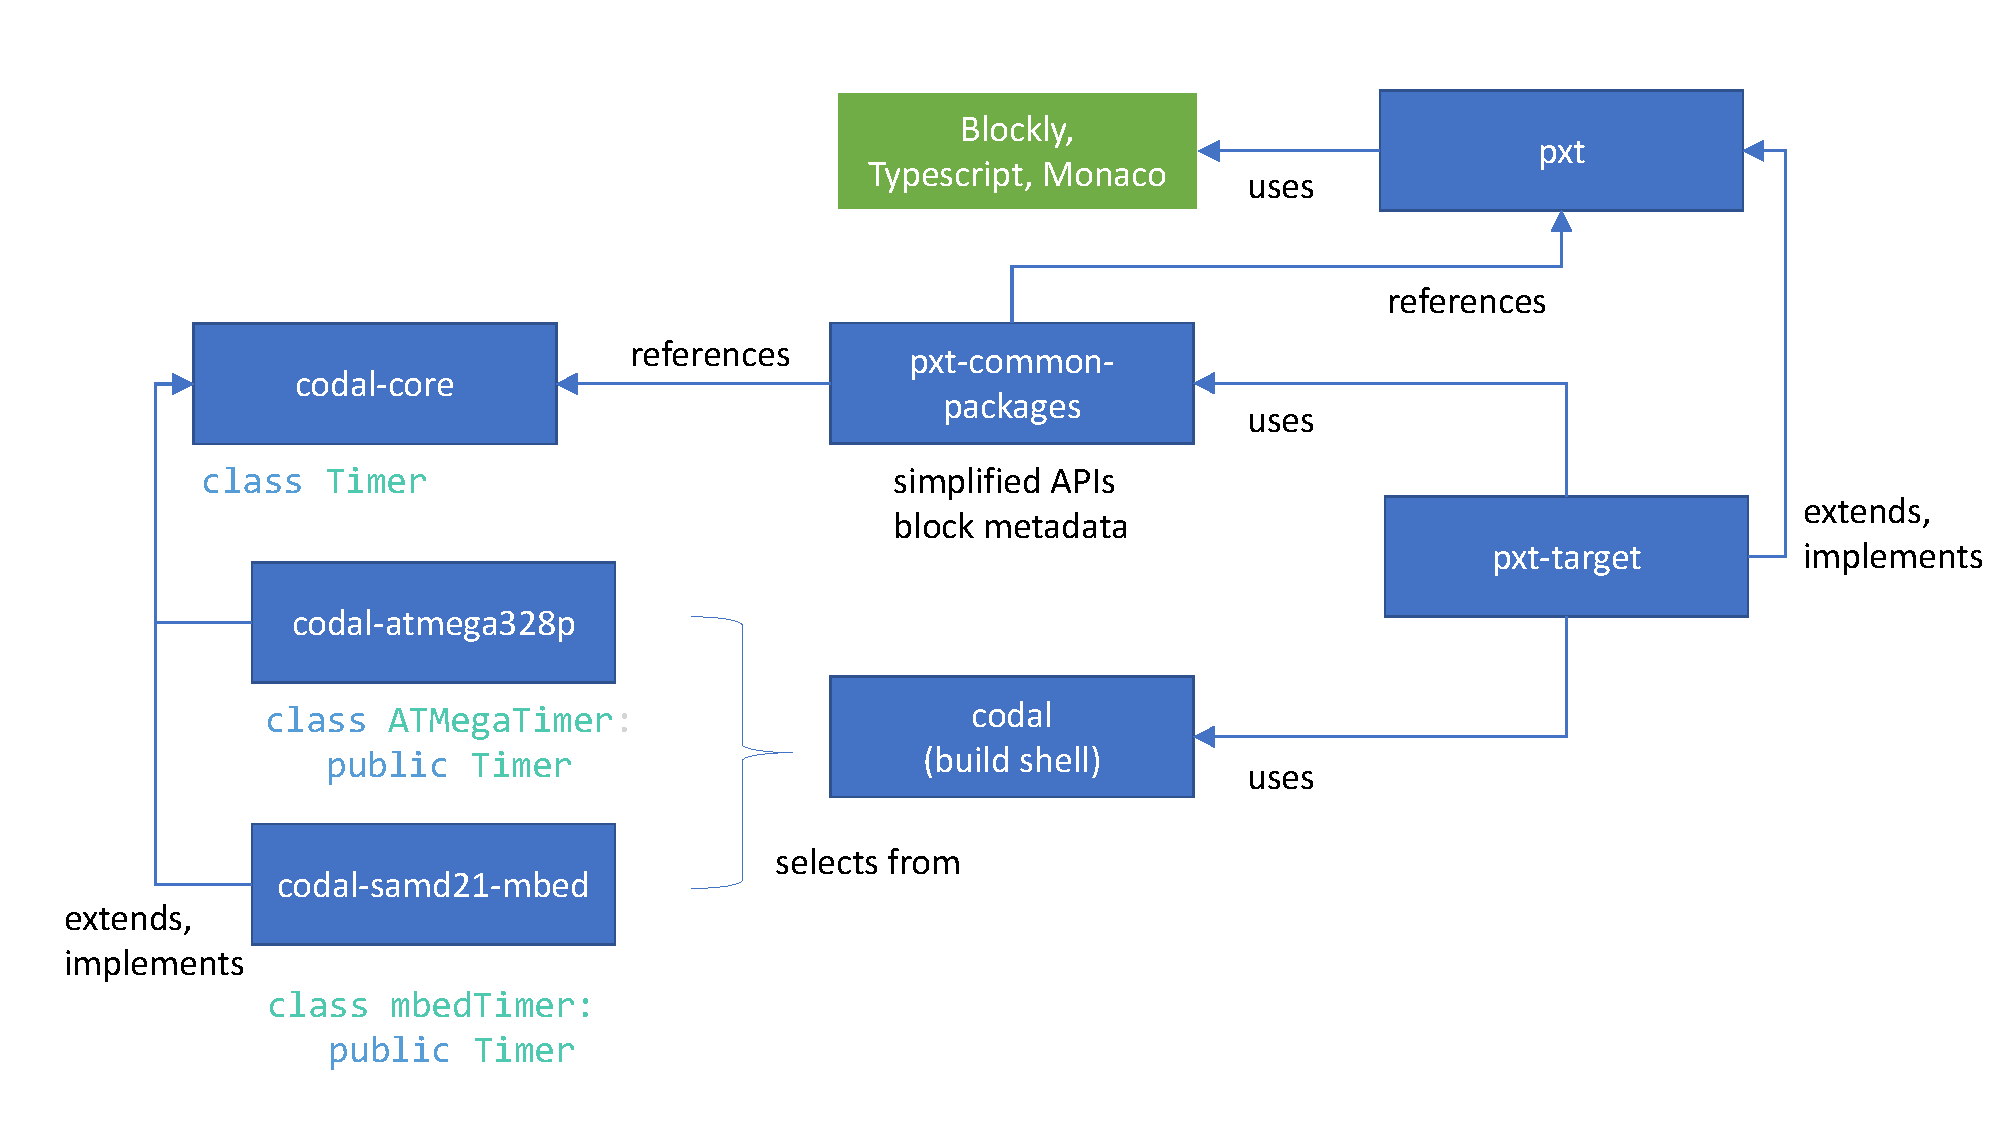
\includegraphics[width=5.5in]{reposFig.pdf}
  \caption{\label{fig:repos}Relationships between platform components/repos. Yellow boxes represent the \MC (PXT) components; blue
  boxes represent the CODAL components; green boxes represent external components.}
\end{figure*}

The platform consists of a stack of four novel technologies, the subject of
this paper. The entry point of the platform is \emph{\MC} (\href{https://makecode.com}{makecode.com}),
a web app that supports both visual block programming and text programming,
via \emph{Static TypeScript}, with conversion 
between the two program representations. The web app has in-browser execution 
via a device simulator, as well as compilation to machine code and linking against a 
pre-compiled C++ runtime (\emph{CODAL}, the Component-oriented Device Abstraction Layer). No C/C++ compiler is invoked to compile user code. 
The result of compilation is a binary file that is ``downloaded'' from the web app to the user's 
computer and then flashed to the microcontroller, with the aid of the \emph{UF2} file format. The other three major technologies in the stack are:
\begin{itemize}

\item \emph{Static TypeScript} is a statically-typed subset of TypeScript (\url{www.typescriptlang.org}), 
a gradually-typed superset of JavaScript, for fast execution on low-memory devices, with
a simple model for linking against pre-compiled C++; 

\item \emph{CODAL} is a C++ library that maps 
each hardware component to one or more software components that communicate via events and
schedule event handlers to run non-preemptively on fibers. 

\item \emph{USB Flashing Format} (UF2) is a new file format designed for flashing microcontrollers over the Mass Storage
Class protocol; the format greatly speeds the installation of user 
programs and is robust to difference in operating systems. 
\end{itemize}
These four advances enable beginners to get started programming microcontrollers from any modern web browser, and enable
hardware vendors to innovate and safely add new components to the mix using Static TypeScript, leveraging its
foreign function interface to C++. 
Once the web app has been loaded, 
all the above functionality works offline (i.e., if the host machine loses its connection 
to the internet).

Platform targets can be seen at \url{www.makecode.com}, where the \MC web app for a variety of boards is available, 
including:
\begin{itemize}
\item the \emph{\href{https://microbit.org}{micro:bit}}, a Nordic nRF51822 microcontroller with Cortex-M0 processor, 256KB flash and 16KB RAM~\cite{microbitICSE2016};
\item Adafruit's \emph{\href{https:/adafruit.com/products/3333}{Circuit Playground Express}}, an Atmel SAMD21 microcontroller with Cortex-M0 processor, 256KB flash and 32KB RAM;
\item the \emph{\href{https://store.arduino.cc/usa/arduino-uno-rev3}{Arduino Uno}}, an Atmel ATmega328 microcontroller with AVR processor, 32KB fLash and 2KB RAM.
\end{itemize}

We encourage the reader to choose a board (from \url{https://makecode.com})
and experiment with programming it, to appreciate the 
qualitative aspects of the platform: its simplicity and ease of use.  In this 
paper, we evaluate quantitative aspects of the platform: 
compilation speed, code size, and runtime performance.  In particular, we evaluate:
\begin{itemize}
\item the compile time of Static TypeScript compile/link of user code (to machine code) with respect 
      to the GCC C/C++ toolchain, as well as the size of the resulting executable;
\item the time to load code onto a microcontroller using UF2, compared to standard bootloaders
      such as Arduino and ARM's DAPlink; 
\item The performance of a set of small benchmarks, written in both Static TypeScript and C++,
      compiled with the \MC and GCC toolchains, as well as the performance of device drivers
      written in Static TypeScript compared to their C++ counterparts;
\item \emph{energy consumption: CODAL vs. Arduino}
[evaluate with respect to the popular Arduino toolset, for boards with 8-bit (AVR) and 32-bit (Cortex-M0) microcontrollers. 
Summary of evaluation]
\item \emph{native code vs. bytecode} For the Arduino Uno, which has the most constrained flash (32KB) and RAM (2KB) of the microcontrollers evaluated, we also
evaluate memory consumption and code performance for our native code generation vs. bytecode generation and interpretation. 
\end{itemize}


\begin{figure*}[t]
      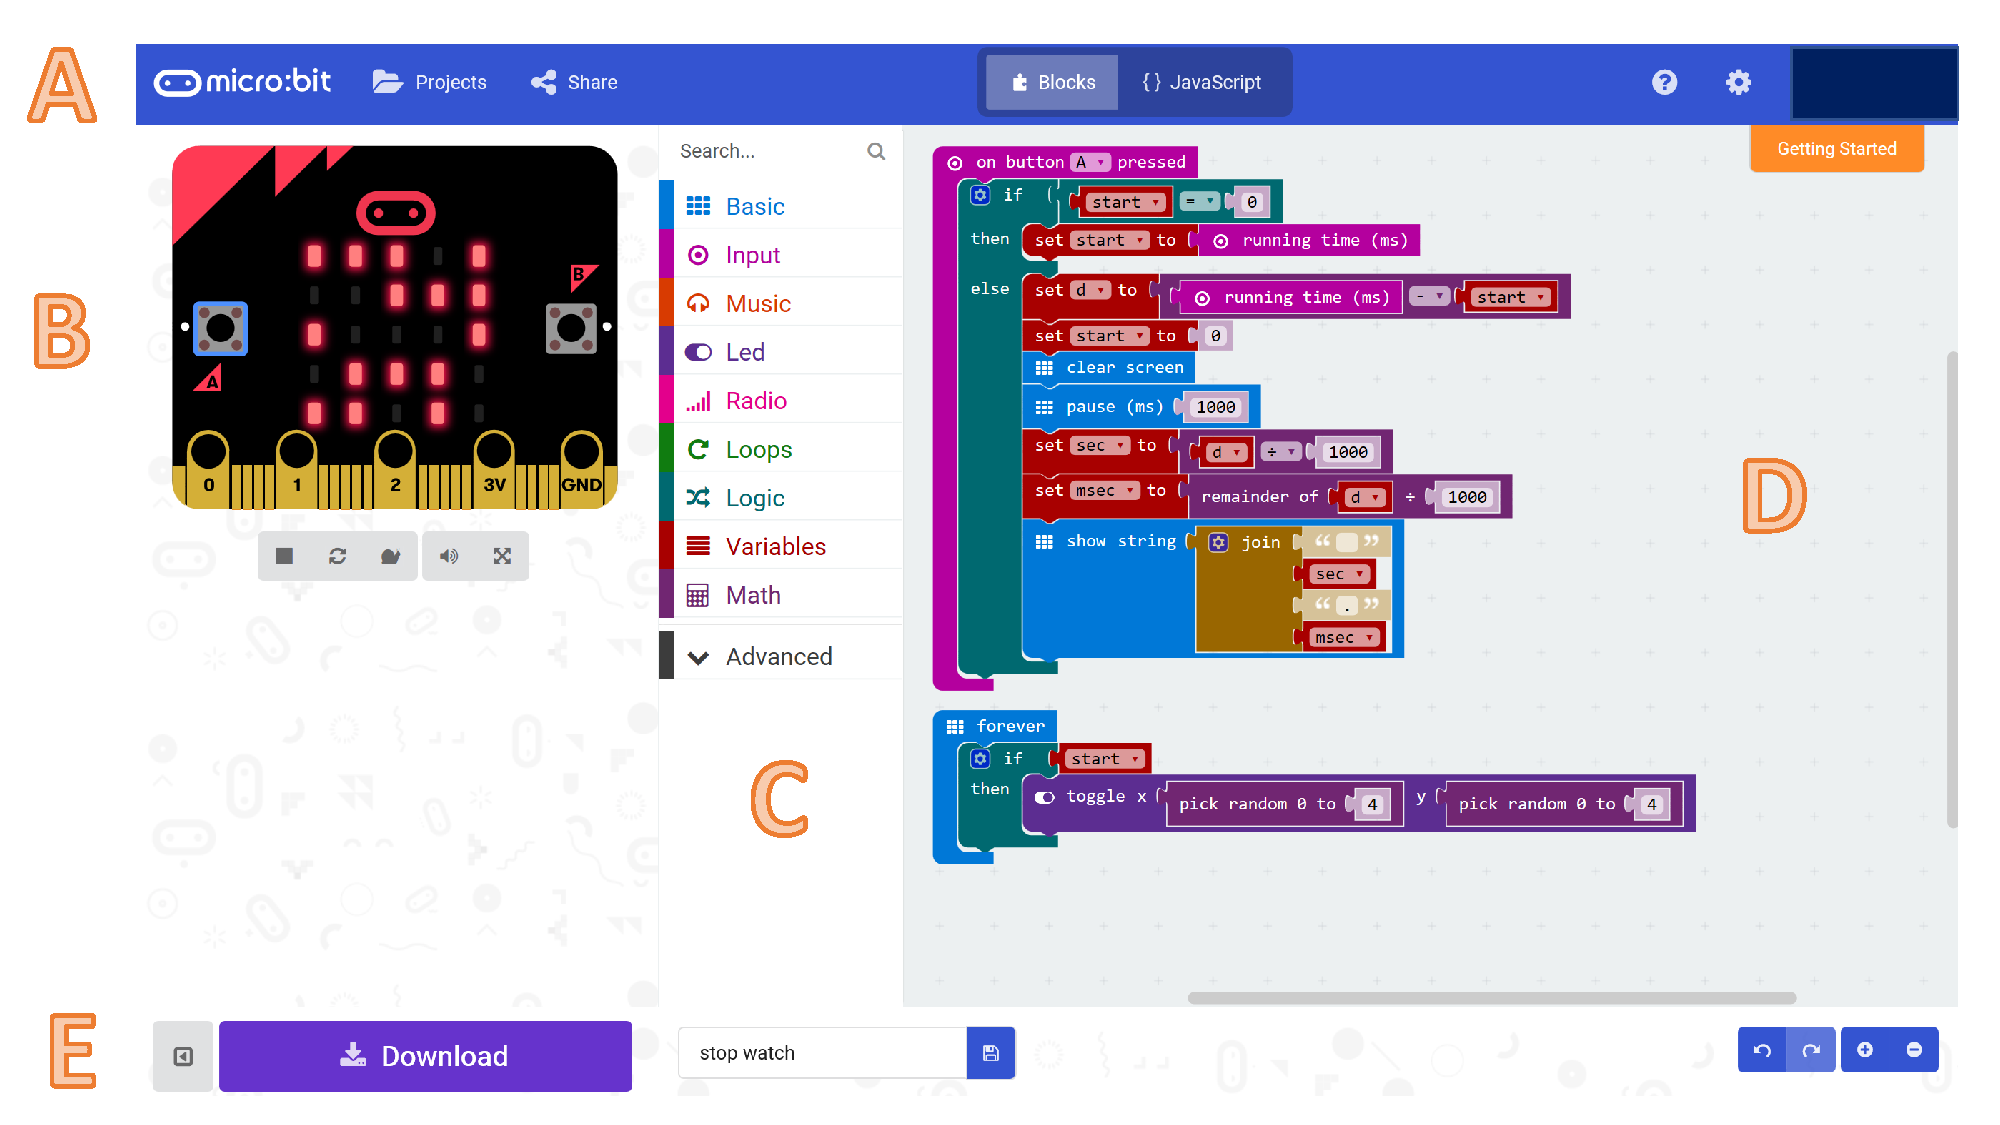
\includegraphics[width=5in]{screenSnapFig.pdf}
  \caption{\label{fig:screenSnap}Screen snapshot of the \MC web app.}
\end{figure*}

All of the platform's components are open source on GitHub
under MIT/Apache licenses. 
Figure~\ref{fig:repos} lists the GitHub repos and the dependences between them. Green boxes represent repos external to the platform (note: not all
repos are represented in the figure).

The \MC framework 
is at \emph{\href{https://github.com/microsoft/pxt}{pxt}} (PXT is the previous codename of \MC). 
A \emph{pxt-target} extends the framework to create an environment for a specific board. Targets
for the three previously mentioned boards are at: 
~\emph{\href{https://github.com/microsoft/pxt-microbit}{pxt-microbit}}, 
~\emph{\href{https://github.com/microsoft/pxt-adafruit}{pxt-adafruit}}, and
~\emph{\href{https://github.com/microsoft/pxt-arduino-uno}{pxt-arduino-uno}}.
The latter two targets make use of a common set of libraries, 
\emph{\href{https://github.com/microsoft/pxt-common-packages}{pxt-common-packages}},
which build upon CODAL's microcontroller independent core abstractions at
~\emph{\href{https://github.com/lancaster-university/codal-core}{codal-core}}.  

Platform- and microcontroller-dependent specialization and optimizations for 
SAMD21 and Atmega328 microcontrollers can be found at
~\emph{\href{https://github.com/lancaster-university/codal-samd21}{codal-samd21}}, 
and
~\emph{\href{https://github.com/lancaster-university/codal-atmega328p}{codal-atmega328p}}.
Not shown in the figure, the SAMD21 repo uses another repo for
MBED-specific optimizations for the Cortex-M0 processor: \emph{\href{https://github.com/lancaster-university/codal-mbed}{codal-mbed}}.

The repo \emph{\href{https://github.com/lancaster-university/codal}{codal}} provides the
tools for compiling a CODAL target.  As can be seen in Figure~\ref{fig:repos}, 
CODAL (the blue boxes) abstracts over platform and microcontroller specific
implementations, while PXT abstracts over programming editors
and languages (Blockly, Monaco, and TypeScript).
The UF2 specification is at~\emph{\href{https://github.com/microsoft/uf2}{uf2}},
with implementations at~\emph{\href{https://github.com/microsoft/uf2-samd21}{uf2-samd21}}
and~\emph{\href{https://github.com/mmoskal/uf2-uno}{uf2-uno}}. These repos are not
shown in the Figure. 
The pxt-microbit target uses a predecessor of the CODAL called the DAL (at
~\emph{\href{https://github.com/lancaster-university/microbit-dal}{microbit-dal}}).

The rest of this paper is organized as follows. Section~\ref{sec:makecode} presents the design and implementation of the \MC framework. 
Sections~\ref{sec:sts},~\ref{sec:codal} and~\ref{sec:uf2} describe Static TypeScript, the CODAL C++ runtime, and the UF2 flashing format,
respectively.  Section~\ref{sec:evaluate} evaluates the performance of the platform and
Section~\ref{sec:related} discusses related work. Finally, Section~\ref{sec:conclude} concludes and speculates about future directions. 
